% TEDO AI Research Lab -- a three-page IEEE conference paper.
% Build: pdflatex paper && bibtex paper && pdflatex paper && pdflatex paper
\documentclass[conference]{IEEEtran}
\IEEEoverridecommandlockouts
\usepackage[T1]{fontenc}
\usepackage{cite}
\usepackage{amsmath,amssymb,amsfonts}
\usepackage{graphicx}
\usepackage{textcomp}
\usepackage{xcolor}
\usepackage{booktabs}
\usepackage{url}
\usepackage{tikz}
\usetikzlibrary{arrows.meta,positioning,fit}
\def\BibTeX{{\rm B\kern-.05em{\sc i\kern-.025em b}\kern-.08em
    T\kern-.1667em\lower.7ex\hbox{E}\kern-.125emX}}

\pdfinfo{
  /Title (TEDO AI Research Lab: A Permissively Licensed Desktop Workbench for Reproducible Machine Learning, Computer Vision and Quantum Simulation)
  /Author (tedo001)
  /Subject (Experiment tracking, reproducibility and Kohn-Sham lattice simulation in a desktop workbench)
  /Keywords (experiment tracking, reproducibility, density functional theory, Kohn-Sham equations, scientific visualization, open-source software)
}

\begin{document}

\title{TEDO AI Research Lab: A Permissively Licensed Desktop Workbench for Reproducible Machine Learning, Computer Vision and Quantum Simulation}

\author{\IEEEauthorblockN{tedo001}
\IEEEauthorblockA{\textit{TEDO AI Research Lab}\\
\url{https://github.com/tedo001/tedo-sim-lab}\\
durgamani.d.e.c.e.50@gmail.com}}

\maketitle

\begin{abstract}
Machine-learning research on a single workstation is usually spread over notebooks, scripts,
terminals and hosted trackers, which makes experiments hard to repeat and leaves licensing and
data-provenance questions open. We present TEDO AI Research Lab, an open-source desktop
workbench built with Qt for Python in which an experiment is one declarative file that runs in a
background worker process, is recorded in SQLite and MLflow, and leaves a run folder with a
reproducibility snapshot from which it can be repeated. The workbench integrates image
classification with PyTorch, eleven scikit-learn and XGBoost models, an interactive CNN
explainer, a network designer, a dataset hub that checks licences at their sources, and a
simulation laboratory for quantum circuits, wave packets and computer vision. Its newest module
solves the Kohn--Sham equations self-consistently for electrons in a two-dimensional crystal
lattice and renders the lattice potential, sampled electrons and averaged density as interactive
three-dimensional views drawn without OpenGL. Every dependency and build tool is permissively
licensed, a rule enforced by the tests. The physics engine reproduces the Madelung energies of the
two-dimensional Wigner crystal to six digits and converges the default lattice in seven iterations
and 0.6~s on a four-core CPU; 574 automated tests pass on Linux and Windows.
\end{abstract}

\begin{IEEEkeywords}
experiment tracking, reproducibility, density functional theory, Kohn--Sham equations,
scientific visualization, open-source software
\end{IEEEkeywords}

\section{Introduction}
A machine-learning (ML) result depends on code, data, hyperparameters and the software
environment; missing environment details and undocumented runs are a common reason results cannot
be repeated~\cite{pineau2021reproducibility}. Notebooks~\cite{kluyver2016jupyter} and experiment
trackers such as MLflow~\cite{zaharia2018mlflow} address parts of this, but a researcher working
alone still moves between many tools, and several popular vision libraries carry copyleft
licences that restrict how derived work may be shared.

TEDO AI Research Lab keeps the whole cycle in one desktop application: choose a dataset and
model, run, track, compare, explain and reproduce, on one machine with a 4~GB GPU. Its
contributions are:
\begin{itemize}
\item an architecture in which every experiment is a strict YAML file run by a worker process
that streams JSON events, recorded in SQLite and MLflow with a reproducibility snapshot;
\item integrated learning laboratories and a dataset hub with a licence policy enforced in code;
\item a simulation laboratory with a self-consistent plane-wave Kohn--Sham
solver~\cite{kohn1965selfconsistent} for two-dimensional lattices and interactive 3-D views;
\item validation of the physics against exact results and of the software by 574 tests on two
operating systems.
\end{itemize}

\section{Related Work}
MLflow~\cite{zaharia2018mlflow} tracks parameters, metrics and artifacts, and Jupyter
notebooks record computations~\cite{kluyver2016jupyter}; the lab uses both inside a local
workbench that also runs the experiments. Training builds on PyTorch~\cite{paszke2019pytorch},
scikit-learn~\cite{pedregosa2011sklearn} and XGBoost~\cite{chen2016xgboost}, with SHAP
values~\cite{lundberg2017shap}. CNN Explainer~\cite{wang2021cnnexplainer} visualises a
convolutional network in the browser; we port its views to a native engine that reproduces
PyTorch's activations exactly. Codes such as Quantum ESPRESSO~\cite{giannozzi2009qe} solve the
Kohn--Sham equations for real three-dimensional materials; our lattice model is a compact
two-dimensional counterpart in which every step of the self-consistent loop can be inspected.

\section{System Architecture}
The code is layered (Fig.~\ref{fig:arch}): \texttt{core} holds contracts and engines without
user-interface code, \texttt{labs} the domain logic, \texttt{plugins} the integrations (Kaggle,
Hugging Face, Roboflow, Colab, MLflow) and \texttt{app} the Qt for Python (PySide6) interface with
29 pages. Tests enforce the import rules and a 400-line limit per module; the system has 286
modules and about 35\,600 lines, with 7\,700 more in tests.

\begin{figure}[t]
\centering
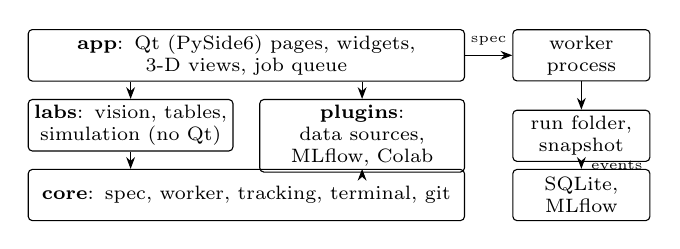
\begin{tikzpicture}[font=\scriptsize, node distance=2.2mm,
  box/.style={draw, rounded corners=1.5pt, align=center, inner sep=2pt, minimum height=6.5mm},
  arr/.style={-{Stealth[length=1.5mm]}, thin}]
\node[box, text width=54mm] (app) {\textbf{app}: Qt (PySide6) pages, widgets,\\3-D views, job queue};
\node[box, text width=24.6mm, below=of app.south west, anchor=north west] (labs)
  {\textbf{labs}: vision, tables,\\simulation (no Qt)};
\node[box, text width=24.6mm, below=of app.south east, anchor=north east] (plugins)
  {\textbf{plugins}: data sources,\\MLflow, Colab};
\node[box, text width=54mm, below=of labs.south west, anchor=north west] (core)
  {\textbf{core}: spec, worker, tracking, terminal, git};
\node[box, text width=16mm, right=6mm of app] (worker) {worker\\process};
\node[box, text width=16mm, right=6mm of plugins] (run) {run folder,\\snapshot};
\node[box, text width=16mm, right=6mm of core] (store) {SQLite,\\MLflow};
\draw[arr] (app.south -| labs) -- (labs);
\draw[arr] (app.south -| plugins) -- (plugins);
\draw[arr] (labs) -- (core.north -| labs);
\draw[arr] (plugins) -- (core.north -| plugins);
\draw[arr] (app) -- node[above, font=\tiny]{spec} (worker);
\draw[arr] (worker) -- (run);
\draw[arr] (run) -- node[right, font=\tiny]{events} (store);
\end{tikzpicture}
\caption{Layers of the workbench and the life of an experiment.}
\label{fig:arch}
\end{figure}

\subsection{Experiments}
A specification names a task, dataset, model, training settings and device; it is validated
strictly and written in canonical form. Launching creates a run folder, and a job queue starts a
worker subprocess that prints one JSON event per line and exits with 0, 1 or 2 for completed,
failed or cancelled; cancellation is cooperative through standard input. Events are recorded in
SQLite with paths relative to the workspace, and the worker mirrors each run to MLflow without
ever failing on a tracking error. A snapshot stores the Python version, platform, packages, git
commit with uncommitted changes and a dataset fingerprint; \emph{Reproduce} queues the same file
as a child run and lists environment differences.

\subsection{Licences, Data and the Interface}
Every dataset and model card carries a licence category checked at its source; downloads
start only when the user asks and gated items are never downloaded. All dependencies and build
tools must be MIT, Apache-2.0, BSD, ISC or PSF licensed, which the tests verify; the one exception
is the LGPL Qt binding, for which no permissive alternative exists. The Windows installer is built
with cx\_Freeze. The interface never blocks: long work runs in worker processes or a thread pool,
and every page is tested to fit half the window.

\section{Laboratories and Simulation}
\subsection{Learning Laboratories}
The vision laboratory trains LeNet-5~\cite{lecun1998gradient}, ResNet-18~\cite{he2016resnet}, a
small CNN and TinyVGG with mixed precision, checkpoints, resumption and early stopping; trained
TinyVGG models open in the CNN explainer. The classical laboratory runs eleven models with
cross-validation, search, ROC curves, permutation importance and SHAP, and a network designer
writes the PyTorch code of a layer stack. The simulation laboratory builds quantum circuits of up
to ten qubits, propagates wave packets by the split-step Fourier method~\cite{feit1982spectral},
generates synthetic COCO-format detection data~\cite{lin2014coco} and models a pinhole camera.

\subsection{Electrons in a Lattice}
Ions of charge $Z$ sit on a square, triangular or honeycomb lattice a height $d$ above a plane
of electrons, which feel $-Z/\sqrt{r^2+d^2}$ from each ion. In Kohn--Sham
theory~\cite{kohn1965selfconsistent} the electrons are described by orbitals $\psi_i$ in an
effective potential (Hartree atomic units),
\begin{equation}
\left[-\tfrac12\nabla^2 + V_{\mathrm{eff}}(\mathbf r)\right]\psi_i = \varepsilon_i\psi_i,\quad
V_{\mathrm{eff}} = V_{\mathrm{ion}} + V_{\mathrm H} + V_{\mathrm{xc}},
\label{eq:ks}
\end{equation}
\begin{equation}
n(\mathbf r) = \sum_i f_i\,|\psi_i(\mathbf r)|^2,\qquad
f_i = \frac{2}{1+e^{(\varepsilon_i-\mu)/k_BT}},
\label{eq:density}
\end{equation}
where $V_{\mathrm H}$ is the Coulomb potential of $n$ itself and $V_{\mathrm{xc}}$ is the local
density approximation of the two-dimensional electron gas: exact exchange and the correlation of
Attaccalite \emph{et al.}~\cite{attaccalite2002correlation}. Orbitals are expanded in plane waves
with $\tfrac12|\mathbf G|^2\le E_{\mathrm{cut}}$ at the $\Gamma$ point of the simulated cell and
the Hamiltonian is diagonalised densely. Fermi smearing~\cite{mermin1965thermal} fixes $\mu$, and
Pulay mixing~\cite{pulay1980convergence} of successive densities is repeated until
$\int|n_{\mathrm{out}}-n_{\mathrm{in}}|\,dA/N<10^{-6}$. The total energy adds an Ewald
sum~\cite{ewald1921berechnung} for the ions and the energy $2\pi dN^2/A$ of the charge sheets.

The electrons on screen are samples of $n(\mathbf r)/N$, not classical particles: walkers take
Metropolis-adjusted Langevin steps~\cite{roberts1996langevin}, so their long-run distribution is
the density, and a walker reaching another ion is drawn as a hop (Fig.~\ref{fig:lattice}).

\begin{figure*}[t]
\centering
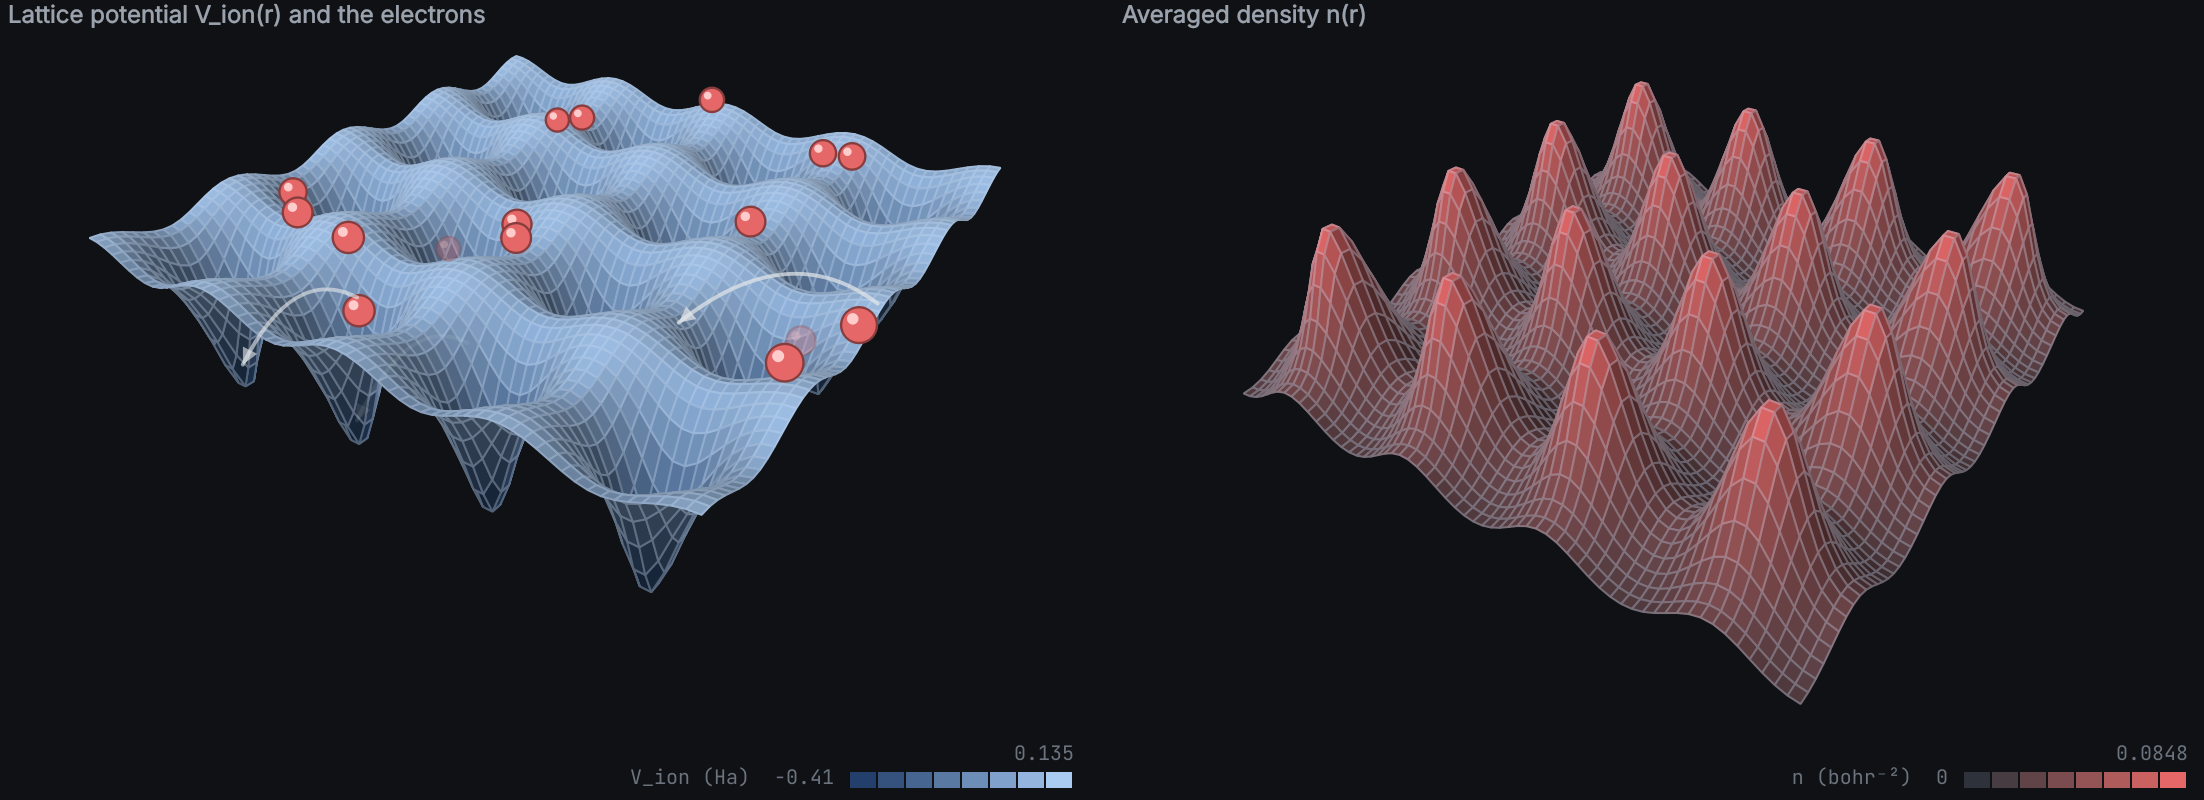
\includegraphics[width=0.84\textwidth]{figures/lattice-3d.png}
\caption{The Lattice tool: (left) the ionic potential $V_{\mathrm{ion}}$ of a $4\times4$ square
lattice with sampled electrons and arrows marking hops between ions; (right) the self-consistent
density $n(\mathbf r)$. Both views are drawn with Qt's 2-D painter and turn together.}
\label{fig:lattice}
\end{figure*}

\subsection{Three-Dimensional Views}
Qt's own 3-D modules are GPL-licensed, so all 3-D views use Qt's 2-D painter: a perspective
orbit camera, shaded quadrilaterals sorted far to near, and a cached image of the static scene
with moving spheres drawn over it. The same camera draws a dataset's rows as a point cloud along
three columns or principal components, coloured by class, in the dataset hub and the results.

\section{Validation}
Table~\ref{tab:verify} compares the engine with independent results. The Ewald sum reproduces
the Madelung energies of the two-dimensional Wigner crystal~\cite{bonsall1977wigner} for any
splitting parameter; the correlation agrees with the fit of Tanatar and
Ceperley~\cite{tanatar1989ground} within 0.6\,\%; plane-wave eigenvalues are variational upper
bounds within $10^{-5}$~Ha of exact diagonalisation on the full grid; and the walkers reproduce the
density to a total variation distance of 0.014. For the default lattice the density change falls
from 0.19 to $1.6\times10^{-7}$ in seven iterations, and raising $E_{\mathrm{cut}}$ from 8 to 20~Ha
changes the energy per electron by $4\times10^{-6}$~Ha. Table~\ref{tab:runs} gives times on a
four-core 2.8~GHz Xeon; $Z=2$ with deeper wells fills the lowest band and opens a gap of 0.236~Ha.

\begin{table}[t]
\caption{Verification Against Exact or Independent Results}
\label{tab:verify}
\centering
\begin{tabular}{@{}lrr@{}}
\toprule
Quantity & Lab & Reference \\
\midrule
Madelung, square ($E r_s/N$, Ha) & $-1.100244$ & $-1.100244$~\cite{bonsall1977wigner} \\
Madelung, triangular & $-1.106103$ & $-1.106103$~\cite{bonsall1977wigner} \\
$\varepsilon_{\mathrm c}(r_s{=}1)$ (Ha) & $-0.11055$ & $-0.11009$~\cite{tanatar1989ground} \\
$\varepsilon_{\mathrm c}(r_s{=}10)$ (Ha) & $-0.03027$ & $-0.03045$~\cite{tanatar1989ground} \\
Sampler total variation & 0.014 & 0 \\
\bottomrule
\end{tabular}
\end{table}

\begin{table}[t]
\caption{Self-Consistent Runs ($4\times4$ Cells, $E_{\mathrm{cut}}=8$~Ha)}
\label{tab:runs}
\centering
\setlength{\tabcolsep}{4pt}
\begin{tabular}{@{}lrrrrr@{}}
\toprule
Lattice & $N$ & Waves & Iter. & Time (s) & $E/N$ (Ha) \\
\midrule
Square & 16 & 509 & 7 & 0.60 & $-0.38247$ \\
Triangular & 16 & 435 & 7 & 0.40 & $-0.37713$ \\
Honeycomb & 32 & 379 & 7 & 0.33 & $-0.22322$ \\
Square, vacancy & 15 & 509 & 15 & 1.08 & $-0.38353$ \\
Square, $Z{=}2$, $d{=}0.6$ & 32 & 509 & 9 & 0.63 & $-1.00024$ \\
\bottomrule
\end{tabular}
\end{table}

The software is checked by 574 automated tests, run on every change on Ubuntu (Python 3.11 and
3.13) and Windows (Python 3.11); a smoke test opens all 29 pages and runs each engine, and the
Windows installer is built, installed silently and started in the same pipeline.

\section{Discussion and Conclusion}
The lattice model is deliberately small: two-dimensional, spin-unpolarised, local-density and
sampled at the $\Gamma$ point only, with at most 1\,600 plane waves; within these limits it exposes
every step of the self-consistent loop. TEDO AI Research Lab shows that one permissively licensed
desktop application can run, track, explain and reproduce ML experiments while hosting physics
simulations verified against exact values. Planned work adds band structures and spin, 3-D views
of learned features, and laboratories for audio and language.

\bibliographystyle{IEEEtran}
\bibliography{references}

\end{document}
